% A0 portrait poster — matches poster_template.pptx layout
\documentclass[20pt]{article}
\usepackage[
  paperwidth=841mm, paperheight=1189mm,
  left=7mm, right=7mm, top=0mm, bottom=0mm
]{geometry}
\usepackage{xcolor}
\usepackage{graphicx}
\usepackage{booktabs}
\usepackage{amsmath}
\usepackage[T1]{fontenc}
\usepackage[utf8]{inputenc}
\usepackage{lmodern}
\usepackage{url}
\pagestyle{empty}
\setlength{\parindent}{0pt}
\setlength{\parskip}{0pt}

% ── Template colours ────────────────────────────────────────────
\definecolor{tmplblue}{RGB}{11,83,148}
\definecolor{tmplbadge}{RGB}{243,243,243}
\definecolor{warn}{RGB}{190,40,20}
\definecolor{good}{RGB}{20,140,50}
\definecolor{accent}{RGB}{0,120,200}
\definecolor{luhgray}{RGB}{215,215,215}

% ── Font sizes (30pt base) ───────────────────────────────────────
\renewcommand{\normalsize}{\fontsize{30}{37}\selectfont}
\renewcommand{\large}{\fontsize{34}{42}\selectfont}
\renewcommand{\Large}{\fontsize{40}{49}\selectfont}
\renewcommand{\LARGE}{\fontsize{48}{58}\selectfont}
\renewcommand{\huge}{\fontsize{62}{74}\selectfont}
\renewcommand{\Huge}{\fontsize{78}{92}\selectfont}
\normalsize

% ── Helpers ─────────────────────────────────────────────────────
% \sectionbox{num}{colour}{title}{body}
\newcommand{\sectionbox}[4]{%
  \noindent
  \colorbox{#2}{\parbox{\dimexpr\linewidth-2\fboxsep}{%
    \vspace{3pt}%
    \makebox[34pt]{\colorbox{tmplbadge}{\makebox[30pt]{\LARGE\bfseries\color{black}#1}}}%
    \enspace{\LARGE\bfseries\color{white}#3}%
    \vspace{5pt}}}\\[-1pt]%
  \colorbox{white}{\parbox{\dimexpr\linewidth-2\fboxsep}{%
    \vspace{12pt}#4\vspace{12pt}}}%
  \vspace{12pt}%
}

% sub-section mini-header inside Key Insights
\newcommand{\minihdr}[2]{%
  \colorbox{#1}{\parbox{\dimexpr\linewidth-2\fboxsep}{%
    \large\bfseries\color{white}\strut\enspace#2\strut}}\\[-1pt]%
  \colorbox{luhgray}{\parbox{\dimexpr\linewidth-2\fboxsep}{%
}}}

% ════════════════════════════════════════════════════════════════
\begin{document}

% ── TOP STRIPE ──────────────────────────────────────────────────
\noindent\colorbox{tmplblue}{\parbox{\linewidth}{\vspace{4mm}}}\par\vspace{8pt}

% ── HEADER ──────────────────────────────────────────────────────
\noindent\hspace{2mm}\parbox{\dimexpr\linewidth-4mm}{%
  {\huge\bfseries
    Curriculum Ordering, Catastrophic Forgetting,\\[10pt]
    and OOD Generalization in PPO Agents}\\[12pt]
  {\LARGE Keisuke Nishioka \enspace$\cdot$\enspace
    Leibniz Universit\"{a}t Hannover, SoSe\,2026}\\[8pt]
  {\large\color{gray}
    Poster Presentations in context of ``Reinforcement Learning'' Lecture
    \quad\url{github.com/keisuke58/LUH_summer_2026}}%
}\par\vspace{8pt}

% ── DIVIDER ─────────────────────────────────────────────────────
\noindent\colorbox{tmplblue}{\parbox{\linewidth}{\vspace{4mm}}}\par\vspace{12pt}

% ── TWO-COLUMN BODY  left=38%  right=60% ────────────────────────
\noindent
\begin{minipage}[t]{0.378\textwidth}

% ── 1. TL;DR ────────────────────────────────────────────────────
\sectionbox{1}{tmplblue}{TL;DR}{%
  \textbf{Q:} Does curriculum ordering help OOD generalization?\\[10pt]
  \textbf{A:}\enspace\textcolor{warn}{\textbf{Progressive is worst}}, both in-dist \emph{and} OOD, due to catastrophic forgetting.\\[10pt]
  \textcolor{good}{\textbf{Diversity}}, not ordering, drives transfer.\\[10pt]
  \textbf{Rec:} Use multi-task (Mixed/Random).
}

\vfill

% ── 3. Approach ─────────────────────────────────────────────────
\sectionbox{3}{tmplblue}{Approach}{%
  \textbf{3 training stages:}\\[7pt]
  \begin{tabular}{ll}
    Easy   & \texttt{Empty-8x8} (dense)\\[3pt]
    Medium & \texttt{FourRooms} (sparse)\\[3pt]
    Hard   & \texttt{KeyCorridorS3R1} (v.\ sparse)
  \end{tabular}\\[14pt]
  \textbf{5 held-out OOD environments:}\\[4pt]
  DoorKey, MultiRoom, SimpleCrossing,\\
  LavaCrossing, DistShift1\\[14pt]
  \textbf{5 conditions $\times$ 10 seeds $\times$ 1M steps}\\[10pt]
  \begin{tabular}{ll}
    \toprule
    \textbf{Condition} & \textbf{Rule}\\
    \midrule
    Progressive & Easy$\to$Mid$\to$Hard ($\tau\!=\!70\%$)\\[3pt]
    Reverse     & Hard$\to$Mid$\to$Easy\\[3pt]
    Random      & Uniform random\\[3pt]
    Hard-only   & Always Hard\\[3pt]
    Mixed       & Multi-task\\
    \bottomrule
  \end{tabular}\\[14pt]
  \textbf{Algorithm:} PPO (stable-baselines3)\\[6pt]
  \textbf{Advance rule:} success rate $\geq\tau$ over 20-episode window\\[6pt]
  \textbf{Stats:} Kruskal--Wallis + Mann--Whitney $U$ (Bonferroni $\alpha\!=\!0.05$)
}

\vfill

% ── 5. Future Works ─────────────────────────────────────────────
\sectionbox{5}{tmplblue}{Future Works}{%
  \begin{itemize}\itemsep10pt
    \item \textbf{Auto-curriculum} [Portelas et al., 2020]:\\
          dynamic difficulty avoids forgetting
    \item \textbf{EWC} [Kirkpatrick et al., 2017]:\\
          regularize stage-transition forgetting
    \item \textbf{Domain randomization}\\
          for principled OOD transfer
    \item Scale to 10M steps, more diverse envs
  \end{itemize}
}

\end{minipage}%
\hspace{0.012\textwidth}%
\begin{minipage}[t]{0.600\textwidth}

% ── 2. Motivation ───────────────────────────────────────────────
\sectionbox{2}{tmplblue}{Motivation \& Problem Setting}{%
  Curriculum learning [Bengio et al., 2009] proposes easy-to-hard ordering to accelerate convergence,
  but whether ordering also promotes \textbf{OOD generalization} [Kirk et al., 2023] is unknown.\\[12pt]
  \begin{tabular}{@{}p{12mm}p{85mm}p{145mm}@{}}
    \toprule
    & \textbf{Hypothesis} & \textbf{Expected}\\
    \midrule
    H1 & Progressive $>$ others in-dist  & Easy$\to$Hard eases learning\\[4pt]
    H2 & Mixed best for OOD              & Diversity promotes transfer\\[4pt]
    H3 & Perf.--gen.\ gap                & Curriculum overfits training\\
    \bottomrule
  \end{tabular}
}

% ── 4. Key Insights ─────────────────────────────────────────────
\sectionbox{4}{tmplblue}{Key Insights}{%

%% Row 1 ──────────────────────────────────────────────────────────
\begin{minipage}[t]{0.485\linewidth}
\colorbox{tmplblue}{\parbox{\dimexpr\linewidth-2\fboxsep}{\large\bfseries\color{white}\strut\enspace In-Distribution Results\strut}}\\[-1pt]
\colorbox{luhgray}{\parbox{\dimexpr\linewidth-2\fboxsep}{%
  \vspace{5pt}%
  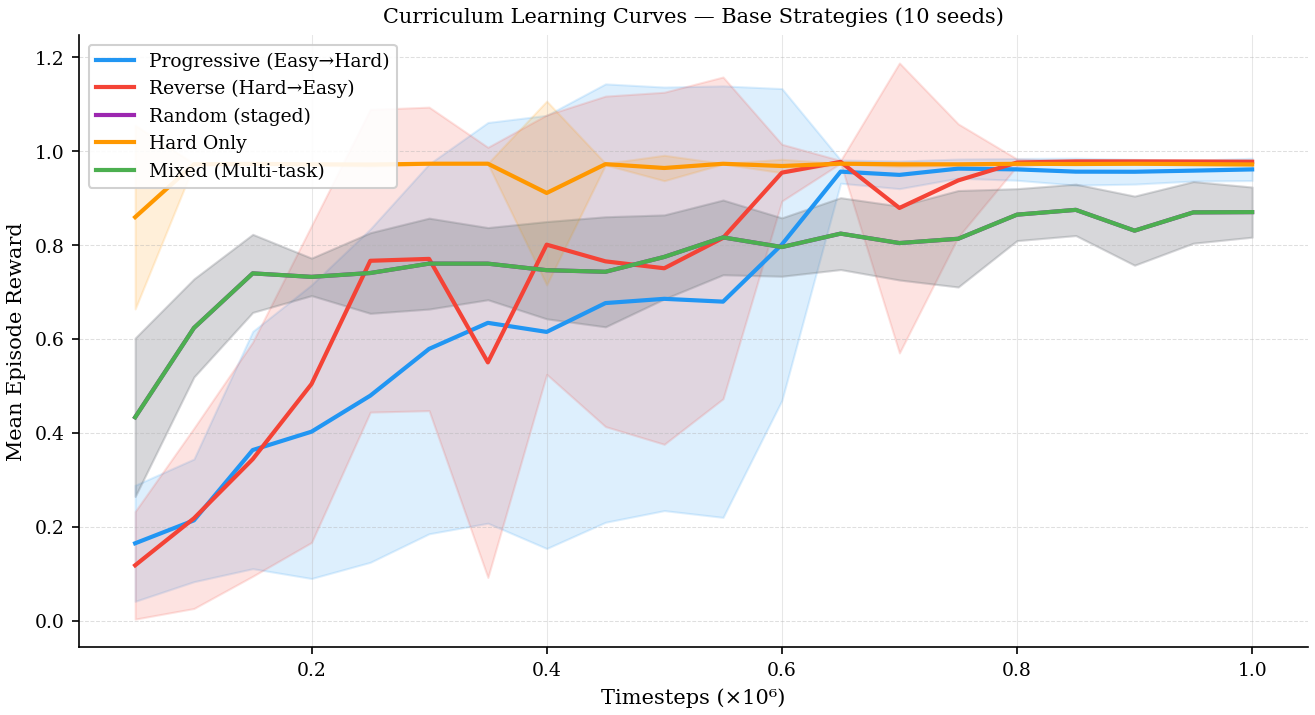
\includegraphics[width=\linewidth,height=195mm,keepaspectratio]{figures/learning_curves.png}\\[4pt]
  {\small\color{gray}\textit{Figure 1: Learning curves (mean $\pm$ std, 10 seeds).}}\\[6pt]
  \begin{tabular}{@{}lcc@{}}
    \toprule
    & \textbf{Train} & \textbf{OOD-SR}\\
    \midrule
    \textcolor{good}{Mixed/Rand} & $0.712$ & $0.059$\\[2pt]
    Reverse      & $0.367$ & $0.075$\\[2pt]
    Hard-only    & $0.332$ & $0.000$\\[2pt]
    \textcolor{warn}{Prog.}  & $0.265$ & $0.004$\\
    \bottomrule
  \end{tabular}\\[6pt]
  \textcolor{warn}{\textbf{Progressive worst}} ($p\!<\!0.001$).%
  \vspace{5pt}}}
\end{minipage}%
\hspace{0.02\linewidth}%
\begin{minipage}[t]{0.485\linewidth}
\colorbox{warn}{\parbox{\dimexpr\linewidth-2\fboxsep}{\large\bfseries\color{white}\strut\enspace Catastrophic Forgetting\strut}}\\[-1pt]
\colorbox{luhgray}{\parbox{\dimexpr\linewidth-2\fboxsep}{%
  \vspace{5pt}%
  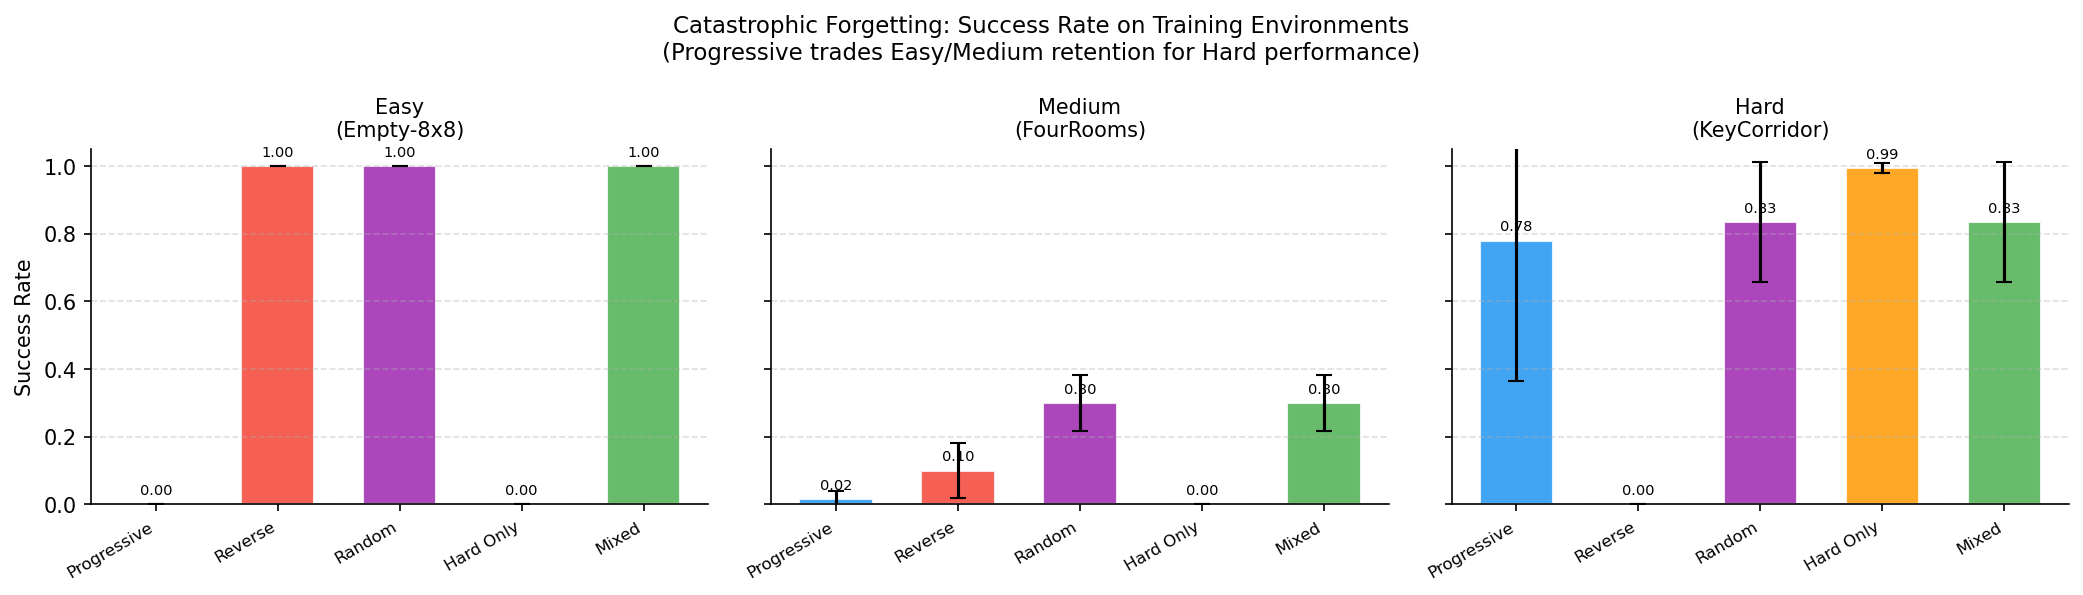
\includegraphics[width=\linewidth,height=195mm,keepaspectratio]{figures/catastrophic_forgetting.png}\\[4pt]
  {\small\color{gray}\textit{Figure 2: Per-stage final reward.}}\\[6pt]
  \begin{tabular}{@{}lrrr@{}}
    \toprule
    & \textbf{Easy} & \textbf{Med} & \textbf{Hard}\\
    \midrule
    \textcolor{warn}{Prog.}  & $0.00$ & $0.02$ & $0.78$\\[2pt]
    Mixed        & $1.00$ & $0.30$ & $0.84$\\[2pt]
    Reverse      & $1.00$ & $0.10$ & $0.00$\\
    \bottomrule
  \end{tabular}\\[6pt]
  Prog.\ forgets Easy/Med entirely.\\
  $\sim$200k steps wasted.%
  \vspace{5pt}}}
\end{minipage}

\vspace{12pt}

%% Row 2 ──────────────────────────────────────────────────────────
\begin{minipage}[t]{0.485\linewidth}
\colorbox{tmplblue}{\parbox{\dimexpr\linewidth-2\fboxsep}{\large\bfseries\color{white}\strut\enspace OOD Generalization\strut}}\\[-1pt]
\colorbox{luhgray}{\parbox{\dimexpr\linewidth-2\fboxsep}{%
  \vspace{5pt}%
  
\includegraphics[width=\linewidth,height=195mm,keepaspectratio]{figures/ood_success_rate.png}\\[4pt]
  {\small\color{gray}\textit{Figure 3: Zero-shot OOD success rate (10 seeds).}}\\[6pt]
  Mixed/Random $\gg$ Hard-only, Progressive on SimpleCrossing ($p\!<\!0.001$).%
  \vspace{5pt}}}
\end{minipage}%
\hspace{0.02\linewidth}%
\begin{minipage}[t]{0.485\linewidth}
\colorbox{accent}{\parbox{\dimexpr\linewidth-2\fboxsep}{\large\bfseries\color{white}\strut\enspace Endpoint Alignment\strut}}\\[-1pt]
\colorbox{luhgray}{\parbox{\dimexpr\linewidth-2\fboxsep}{%
  \vspace{8pt}%
  \textbf{Reverse 30\% on DistShift1:}\\[5pt]
  Ends on Easy $\Rightarrow$ open-room policy\\
  DistShift1 $=$ open-room, shifted obs\\
  $\Rightarrow$ \textbf{coincidental transfer}\\
  ($\sigma\!=\!0.48$, unreliable)\\[14pt]
  \textbf{Progressive 0\% everywhere:}\\[5pt]
  Ends on Hard $\Rightarrow$ key-door specialist\\
  No OOD env needs this exact skill\\
  $\Rightarrow$ \textbf{zero transfer}%
  \vspace{8pt}}}
\end{minipage}

\vspace{12pt}

%% Row 3 ──────────────────────────────────────────────────────────
\begin{minipage}[t]{0.485\linewidth}
\colorbox{tmplblue}{\parbox{\dimexpr\linewidth-2\fboxsep}{\large\bfseries\color{white}\strut\enspace OOD Gap Analysis\strut}}\\[-1pt]
\colorbox{luhgray}{\parbox{\dimexpr\linewidth-2\fboxsep}{%
  \vspace{5pt}%
  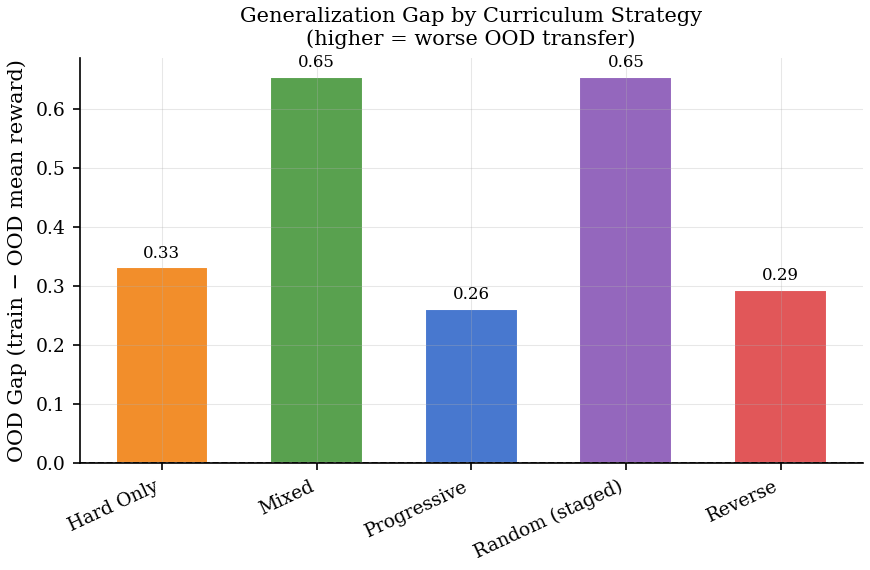
\includegraphics[width=\linewidth,height=195mm,keepaspectratio]{figures/ood_gap_bar.png}\\[4pt]
  {\small\color{gray}\textit{Figure 4: OOD gap = train $-$ OOD reward.}}\\[6pt]
  Prog.\ small gap $\neq$ good generalisation.\\
  Mixed/Random: best OOD, moderate gap.%
  \vspace{5pt}}}
\end{minipage}%
\hspace{0.02\linewidth}%
\begin{minipage}[t]{0.485\linewidth}
\colorbox{tmplblue}{\parbox{\dimexpr\linewidth-2\fboxsep}{\large\bfseries\color{white}\strut\enspace Transfer (Fine-tuning)\strut}}\\[-1pt]
\colorbox{luhgray}{\parbox{\dimexpr\linewidth-2\fboxsep}{%
  \vspace{5pt}%
  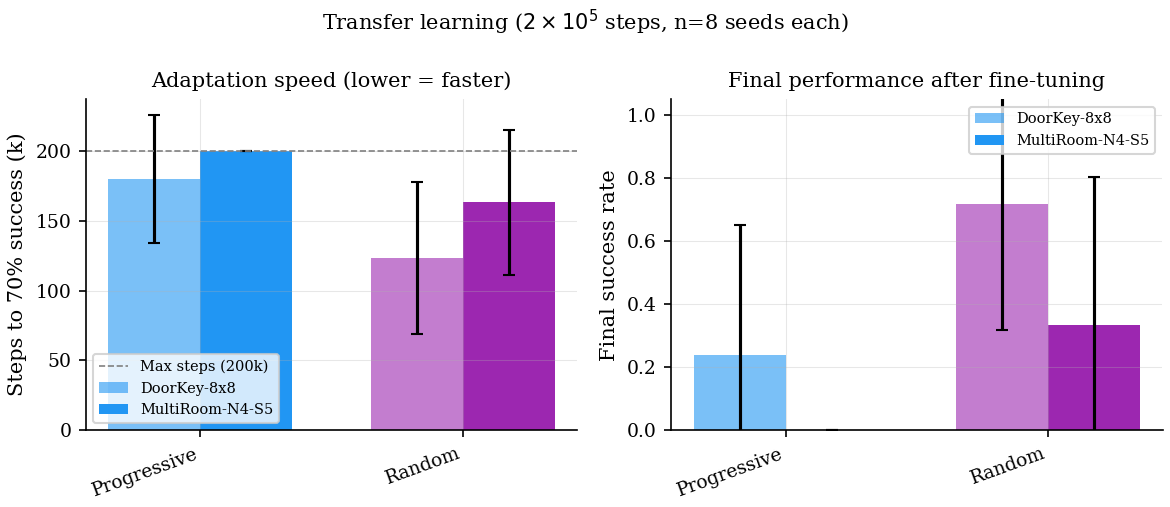
\includegraphics[width=\linewidth,height=195mm,keepaspectratio]{figures/transfer_adaptation.png}\\[4pt]
  {\small\color{gray}\textit{Figure 5: Steps to 70\% on DoorKey-8x8.}}\\[6pt]
  Fine-tuned on DoorKey-8x8.\\
  Random: 70\% in $\sim$85k steps (\textbf{10/10 seeds}).\\
  Progressive: 2/10 seeds only.%
  \vspace{5pt}}}
\end{minipage}

}% end Key Insights body

\end{minipage}

% ── BOTTOM STRIPE ───────────────────────────────────────────────
\vfill
\noindent\colorbox{tmplblue}{\parbox{\linewidth}{%
  \vspace{6pt}\centering
  {\LARGE\bfseries\color{white}
    Key Takeaway:\enspace
    Environment \emph{diversity}, not curriculum ordering, drives performance and OOD generalization.
    Use multi-task training.}%
  \vspace{6pt}}}

\end{document}
